\documentclass[12pt]{article}
\usepackage{amsmath}
\usepackage{graphicx}
\setlength\parindent{0pt}

%opening
\title{Problem Set 2}


\begin{document}

\maketitle


\section*{1}
The key point here is to construct a set of utility functions when the assumptions of market clearing and agents are maximizing their utilities can't hold simultaneously. Consider there is a non-convex part in the indifference curves of both agents, then conceptually, there could be two different points in which both mark clears and utilities are maximized. But with a slight twitch of the indifference, we can make it the case when these two assumptions cannot hold the same time as in the figure. 
\begin{figure}[h]
	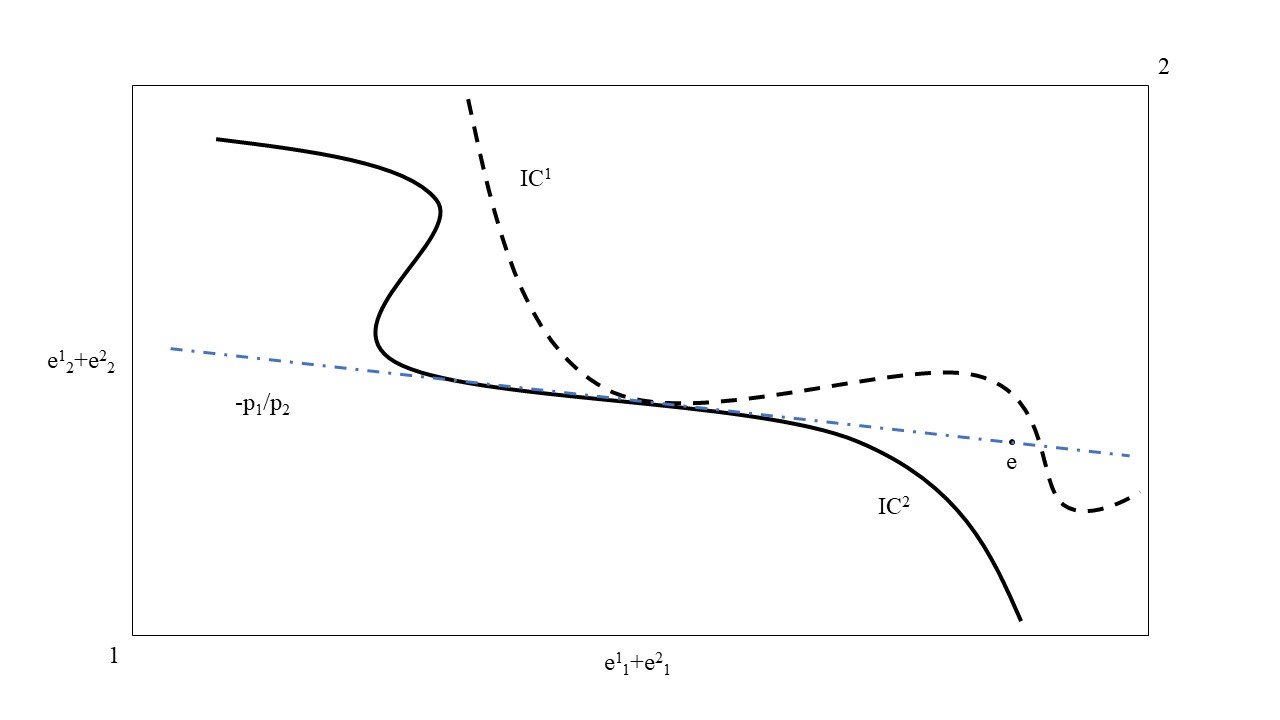
\includegraphics[width=\linewidth]{1_fig.jpg}
	\centering
	\caption{Non-existence of Competitive Equilibrium}
\end{figure}

\section*{3}
(a) One way to interpret the Pareto efficient allocations is to consider the case in which one agent tries to maximize his or her utility when the level of the other agent's utility is fixed. This is captured by the following problem,
\begin{gather*}
\max \quad x_1^1x_2^1\\
s.t. \quad (21-x_1^1)(10-x^1_2)^2=u^2, x^1_1, x^1_2\geq 0
\end{gather*}
By solving this problem we get
\begin{equation*}
x^1_2=\frac{10x^1_1}{42-x^1_1}
\end{equation*}
Therefore, the set of Pareto efficient allocations would be
\begin{equation*}
P(\mathcal{E})=\{(x^1_1,x^1_2),(x^2_1,x^2_2)\in\Re_+|x^1_1\in[0,21], x^1_2=\frac{10x^1_1}{42-x^1_1}, x^2_1=21-x^1_1, x^2_2=10-\frac{10x^1_1}{42-x^1_1}\}
\end{equation*}\\
\\
(b) In a simple two agent model, in the core, each agent would be better off if they engage in the trade rather than consuming their endowments. So the core would be
\begin{equation*}
C(\mathcal{E})=P(\mathcal{E})\cap\{(x^1_1,x^1_2),(x^2_1,x^2_2)\in\Re_+|x^1_1x^1_2>72, x^2_1(x^2_2)^2>108\}
\end{equation*}\\
\\
(c) The definition of competitive equilibrium implies that each agent is maximizing their utilities facing the same price. So we get the first order conditions for both agents as
\begin{equation*}
\frac{x^1_1}{x^1_2}=\frac{p_2}{p_1},\quad \frac{x^2_1}{2x^2_2}=\frac{p_2}{p_1}
\end{equation*}
By combining the budget constraint, first order conditions, and feasibility conditions
\begin{gather*}
\frac{x^1_1}{x^1_2}=\frac{p_2}{p_1},\quad \frac{x^2_1}{2x^2_2}=\frac{p_2}{p_1}\\
p_1x^1_1+p_2x^1_2=18p_1+4p_2,\quad p_1x^2_1+p_2x^2_2=3p_1+6p_2\\
x^1_1+x^2_1=21,\quad x^1_2+x^2_2=10
\end{gather*}
We get the ration of equilibrium price as $\frac{p_1}{p_2}=\frac{4}{11}$, and the equilibrium allocation as $(x^1_1,x^1_2)=(\frac{29}{2},\frac{58}{11})$ and $(x^2_1,x^2_2)=(\frac{13}{2},\frac{52}{11})$\\
\\
(d) We only have to calculate the utility of each agent at equilibrium.
\begin{equation*}
u^1\approx 76.5>72,\quad u^2\approx 145.2>108
\end{equation*}
So the equilibrium allocation is in the core.

\section*{5}
\emph{Theorem 1.2}: First we show that such function can represent the underlying preference. Because $f$ is a strictly increasing function and $u$ has already represents such preference, for any $x^0$ and $x_1$ in $\Re_+^n$, we have $x^0\succeq x^1\Leftrightarrow u(x^0)\geq u(x^1)\Leftrightarrow f(u(x^0))\geq f(u(x^1))\Leftrightarrow v(x^0)\geq v(x^1)$. Therefore, $v$ can represent such preference.\\
\\
Then we want to show that if $v$ can represent such preference, $f$ must be strictly increasing: i.e. $y\geq z\Leftrightarrow f(y)\geq f(z)$. We can divide this requirement into two parts,
\begin{equation*}
y=z\Leftrightarrow f(y)=f(z),\quad y>z\Leftrightarrow f(y)>f(z)
\end{equation*}
For the first part the proof is trivial, because we can always construct such $f$ to satisfy such condition. For the second part, suppose there exists $y$ and $z$ such that $y>z\Leftrightarrow f(y)<f(z)$, then let $y=u(x^0)$ and $z=u(x^1)$
\begin{equation*}
y=u(x^0)>u(x^1)=z\Leftrightarrow v(x^0)<v(x_1)
\end{equation*}
But this is contradicted with the representation of $u$ and $v$, since $u(x^0)>u(x^1)\Leftrightarrow x^0\succeq x^1$ but $v(x^0)<v(x_1)\Leftrightarrow x^0\preceq x^1$\\
\\
\emph{Theorem 1.3}: For $1$, if $u$ is strictly increasing, by the definition of utility function, for any $x^0$ and $x^1$ such that
\begin{align*}
x^0\geq x^1\Rightarrow u(x^0)\geq u(x^1)\Leftrightarrow x^0\succeq x^1\\
x^0>x^1\Rightarrow u(x^0)>u(x^1)\Leftrightarrow x^0\succ x^1
\end{align*}
Hence, $\succeq$ is strictly monotonic. For the only if part, one can just reverse the $\Rightarrow$ into $\Leftarrow$ and finish the proof.\\
\\
For $2$, if $u$ is quasi-concave and $x^0$, $x^1$ are the same as above, by definition, we would have
\begin{equation*}
u\left(tx^0+(1-t)x^1\right) \geq \min \left\{u\left(x^0\right), u\left(x^1\right)\right\}=u(x^1), \forall t \in[0,1]
\end{equation*}
which is equivalent to 
\begin{equation*}
tx^0+(1-t)x_1\succeq x^1, \forall t \in[0,1]
\end{equation*}
Hence, the preference is convex. For the only if part, one only has to reverse the step in the previous proof.\\
\\
For $3$, by the definition of strict quasi-concavity, we get
\begin{equation*}
u(tx^0+(1-t)x^1)>u(x^1)\Leftrightarrow tx^0+(1-t)x^1\succ x^1, \forall t\in[0,1]
\end{equation*}
Hence, the preference is strictly convex. For the only if part, one only has to reverse the step in the previous proof.

\section*{5.7}
(a) It is obvious that $z$ is continuous in each argument. By calculating $z(p_1,p_2)(p_1,p_2)^T=0$, we know that condition 2 is also satisfied. Suppose $\mathbf{p}^{m} \:\text{converges to }\: \overline{\mathbf{p}} \text { where } \overline{p}_{1}=0 \text { but } \overline{p}_{2}>0$, we get
\begin{equation*}
\begin{array}{l}{z_{1}\left(p_{1}^{m}, p_{2}^{m}\right) \rightarrow z_{1}\left(\overline{p}_{1}, \overline{p}_{2}\right)=-1} \\ {z_{2}\left(p_{1}^{m}, p_{2}^{m}\right) \rightarrow z_{2}\left(\overline{p}_{1}, \overline{p}_{2}\right)=0}\end{array}
\end{equation*}
Therefore, neither $z_1$ or $z_2$ is unbounded from above, the condition 3 is not satisfied.\\
\\
(b) Note that no matter what $p_1$ or $p_2$, $z_1$ is always $-1$, so that there is no $(p_1^*,p_2^*)\gg (0,0)$ such that $z(p_1^*,p_2^*)=(0,0)$

\end{document}